\newpage

\section{Theorie}
\subsection{OpenSSL}
OpenSSL umfasst Implementierungen der Netzwerkprotokolle und verschiedener
Verschlüsselungen sowie das Programm openssl für die Kommandozeile zum Beantragen, 
Erzeugen und Verwalten von Zertifikaten. Die in C geschriebene Basisbibliothek stellt allgemeine 
kryptographische Funktionen zum Ver- und Entschlüsseln sowie diverse weitere Werkzeuge bereit.
\footnote{Quelle: \url{https://de.wikipedia.org/wiki/OpenSSL}}


\subsection{AES}
Beim \textbf{Advanced Encryption Standard}handelt sich um ein symmetrisches Verschlüsselungsverfahren, d. h. 
der Schlüssel zum Ver- und Entschlüsseln ist identisch. Der Rijndael-Algorithmus besitzt variable, voneinander unabhängige Block- und 
Schlüssellängen von 128, 160, 192, 224 oder 256 Bit. Rijndael bietet ein sehr hohes Maß an Sicherheit; erst mehr als zehn Jahre nach seiner 
Standardisierung wurde der erste theoretisch interessante, praktisch aber nicht relevante Angriff gefunden.
\\
\\
AES schränkt die Blocklänge auf 128 Bit und die Wahl der Schlüssellänge auf 128, 192 oder 256 Bit ein. Die Bezeichnungen der
drei AES-Varianten AES-128, AES-192 und AES-256 beziehen sich jeweils auf die gewählte Schlüssellänge. AES ist frei verfügbar 
und darf ohne Lizenzgebühren eingesetzt sowie in Soft- und Hardware implementiert werden.\footnote{Quelle: \url{https://de.wikipedia.org/wiki/Advanced_Encryption_Standard}}


\newpage
\section{Erstes - Programm}
\lstinputlisting[language=C, style=StyleC, caption=alt-main.c, captionpos=b, label=alt-main.c]{../../openssl/openssl-Programm/alt/main.c}
\lstinputlisting[language=C, style=StyleC, caption=alt-EVP.c, captionpos=b, label=alt-EVP.c]{../../openssl/openssl-Programm/alt/EVP.c}
\subsubsection{Programm Output:}
\begin{figure}[!htb]
    \centering
    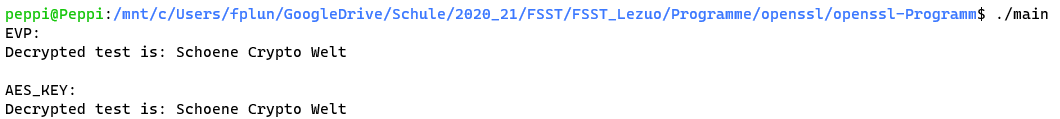
\includegraphics[width=\linewidth]{Programm-Output.png}
    \caption{Programm-Output}
    \label{caption:Programm-Output}
\end{figure}

\newpage
\section{Finales Programm als kleines Command line tool}
\lstinputlisting[language=C, style=StyleC, caption=main.c, captionpos=b, label=main.c]{../../openssl/openssl-Programm/main.c}
\lstinputlisting[language=C, style=StyleC, caption=Encryption.c, captionpos=b, label=Encryption.c]{../../openssl/openssl-Programm/Encryption.c}
\lstinputlisting[language=C, style=StyleC, caption=FileInput.c captionpos=b, label=FileInput.c]{../../openssl/openssl-Programm/FileInput.c}

\subsection{Programm Output:}
\begin{figure}[!htb]
    \centering
    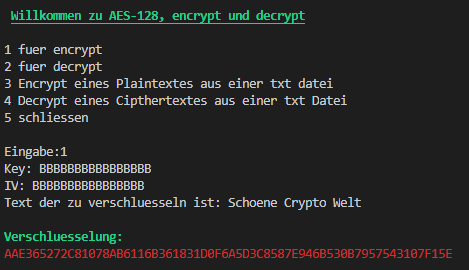
\includegraphics[scale=0.70]{Programm Output.png}
    \caption{Programm Output}
    \label{caption:Programm Output}
\end{figure}






